% !TeX root = ./ada.tex
\providecommand{\relativeRoot}{.}
\documentclass[\relativeRoot/ada.tex]{subfiles}
\graphicspath{
    {\subfix{\relativeRoot/graphics/}}
    {\subfix{\relativeRoot/tikz_graphics/}}
}

\begin{document}

\twocolumn


\section{Introduction}

Radiotherapy aims to use ionising radiation to damage and destroy cancerous tissue. The MR-Linac generates photons with an energy of up to $6$ MeV by accelerating electrons onto a target, where they collide and are decelerated. This process results in the production of a beam of bremsstrahlung from the high kinetic energy of the electrons \cite{klueter_technical}. During their interaction with matter, photons ionise molecules within cells. The ionised electrons are responsible for most of the biological damage caused by radiation. This is because these electrons can cause further ionisations in the molecules they collide with, as they move through the tissue \cite{barrett_practical}.

Ionising radiation can induce lethal cell damage by forming highly reactive radicals inside the cell nucleus that chemically break bonds in molecules. Damages may cause loss of reproducibility or even inflict apoptosis in targeted cells. In general both malignant and benign cells are exposed to radiation in radiotherapy treatment and thus both experience former effects. Much of the motivation for improving the technology of radiation therapy stems from the desire to increase normal tissue complication sparing. This means maintaining functional integrity of irradiated normal tissue and reducing prevalence of normal tissue complication occurrence. There are two elements to the strategy of normal tissue sparing. First element is the existence of a difference in the radiation response of benign and malignant cells. In treatments this difference allows preservation of functional integrity in normal tissue included in the target volume. Difference in this response between malignant and benign cells is assumed to be due to repair kinetics and cell repopulation. To exploit this differential effect the dose is fractionated, that is delivered in small daily increments. Second element of the strategy which is not further discussed here involves the reduction of the dose delivered to normal tissues that are spatially separated from the tumor. \cite{goitein_oncology}

Fractionated therapy is an important rationale for local therapy. Employing fractionation, normal tissue can tolerate higher doses allowing the therapeutic ratio to be increased. One problem of fractionated therapy is that daily treatment over an extended period can result in changes to the geometry of non-stationary organs such as the intestines. Motion of tumors and organs at risk (OAR) in between fractions greatly impairs dose conformity and is generally assumed to degrade the quality of treatments. To account for impaired conformity caused by motion, the target volume can be extended with a safety margin. Safety margins in turn worsen the trade-off between tumor coverage and normal tissue sparing that would be feasible without motion \cite{van_herk_correctdose}. To understand the target volume definition and their extensions one has to understand how treatment plans for irradiation are created.



\section{Theory}

\subsection{Treatment Planning}

To develop an irradiation plan for radiotherapy, it is first necessary to identify and segment the tumor from normal tissue. This is typically done using computed tomography (CT) scans, which provide detailed anatomical information and electron density information that can be used to calculate dose. In some cases, additional imaging modalities such as magnetic resonance (MR) and positron emission tomography (PET) may be used to improve the accuracy of tumor localisation and differentiation from normal tissue with similar density. Once the tumor has been identified and outlined, it is expanded to create specific target volumes that are nested within one another. \cite{barrett_practical}

The gross tumor volume (GTV) represents the primary tumor mass as seen on clinical examination or imaging. Extending the GTV results in the clinical target volume (CTV), which includes any additional microscopic disease. The final extension is the planning target volume (PTV), which accounts for potential errors in positioning during treatment or changes in the size or shape of the tumor or organs. In case no additional CT or MR scans are taken during the course of treatment (which can span several weeks), the PTV margin is essential to account for any uncertainties that may arise due to geometric variations. In addition to outlining the target volumes, it is also necessary to identify and outline any organs at risk (OARs) during treatment planning. OARs are defined as "those normal tissues which lie adjacent to tumors and may therefore be included within treated volumes, with a risk that the radiation may impair their normal functioning" \cite{barrett_practical}. These organs may overlap with the PTV, which can significantly constrain the tumor prescription dose in order to avoid damaging the OAR. There may also be multiple OARs in proximity to the target volume, each of which imposes its own dose constraints.

Once the tumor and OARs have been outlined, an optimal dose distribution can be calculated. This process involves setting constraints and objectives based on the prescribed tumor dose and OAR dose limits. Under a given set of beam angles and interaction model, an optimisation algorithm is used to compute the optimal achievable dose distribution. \cite{wu_reoptimisation}

\subsection{Image guided radiotherapy}

Central to the advances in radiotherapy delivery is the development of medical imaging technologies that provide the 3D delineation of the target volumes and OAR. The development of state-­of-­the-­art imaging methods have enabled modern radiotherapy to develop into a highly personalised, tailored treatment \cite{jaffray_imageguided}. Technologies for image guided radiotherapy include CT, MRI, and PET imaging, where MR images offers superior soft-tissue contrast compared to CT \cite{acharya_onlinemrguided}. Image functionalities provide additional information, that can be used to confirm patient positioning, monitor and mitigate anatomical changes. This enables conforming the treatment plan to new patient geometry \cite{jaffray_imageguided}. However, the conformal dose distribution is only achieved on the reference image which is the planning image, a snapshot of patient anatomy. Inter-fractional and intra-factional anatomy changes from the planning image may deteriorate the dose conformity in actual delivered dose distribution \cite{seungjong_deformable}. The use of more frequent on-line imaging, such as cone beam computerised tomography \cite{jaffray_conebeam} and integrated magnetic resonance imaging \cite{lagendijk_integration}, allows to detect these anatomic changes and aid in correcting or minimising the effect of changes in geometry. Image guidance is used to define the target more accurately and helps minimising the margins of the PTV which give rise to stereotactic body radiotherapy \cite{guckenberger_escalate}. In each fraction through the course of the SBRT treatment at our MR-Linac, the patient is imaged with MRI. The MR image is aligned with deformable image registration to the reference planning CT image. In the presence of large geometry changes compared to reference it is decided whether the dose plan needs to be reoptimised to ensure dose conformity.

\subsection{Uniform Fractionation}

As mentioned before one strategy of normal tissue sparing involves fractionation. In uniform fractionation the prescribed dose is divided into dose fractions of equal size, which are delivered in multiple sessions. To enable comparison between different fractionation schedules the biological effective dose (BED) model is used. More precisely, BED allows determining iso-effective dose fractionation schedules. It is regarded as a measure of the biological dose delivered by a particular combination of equal dose per fraction $D/n$ and total dose $D$ in $n$ fractions to a given tissue \cite{jones_bedrole}. It is defined as
\begin{equation*}
	B = D\left(1+\frac{D / n}{\alpha / \beta}\right)
\end{equation*}

where $\alpha$ and $\beta$ are coefficient that stem from the Track-Event-Model which in low dose regions in approximated with the BED model. The $\alpha / \beta$ ratio is a measure the repair capability : cells with a high $\alpha / \beta$ values respond earlier i.e. show reactions such as proliferative impairment or loss of function earlier. Thus, two adjacent tissues with different $\alpha / \beta$ ratio values, each receiving the same dose and fractionation, will be associated with different BEDs. This does not necessarily mean that one tissue sustains more biological damage than the other. \cite{jones_bedrole}

\section{Prior Work}

Fractionated therapy typically delivers equal dose in every fraction to the tumor when treated with uniform fractionation. Since the plan is fractionated and treatment spans several days or weeks, inter-fractional motion arises. This motion is seen as a handicap to treatments as it can degrade the quality of dose plans and calls for mitigation strategies such as adaptive radiotherapy. Rather than viewing inter-fractional motion as a handicap, it can be seen as an opportunity: the variation in geometry due to motion may be exploited to achieve better treatment quality compared to uniform fractionation.

\subsection{Concept}
Adaptive Fractionation \cite{lu_adaptI}\cite{chen_adaptII}\cite{ramakrishnan_adaptIII} is one approach to exploit inter-fractional motion. In a recently published work from Pérez Haas et al. \cite{perezhaas_adaptive} an approach to adaptive fractionation has been devised and demonstrated with patient data from an MR-Linac.
Adaptive Fractionation extends the existing adaptive therapy paradigm to modification of the tumor dose in each fraction: the dose is increased on favourable treatment days, i.e. when the distance between tumor and dose-limiting OAR is relatively large; and the dose is reduced for unfavourable geometries, i.e. when the tumor and OAR are closer. Thereby, the ratio between total dose delivered to the OAR versus total dose delivered to the tumor may be improved compared to uniform treatments that deliver the same dose in each fraction \cite{perezhaas_adaptive}. In the following the preliminary work is explained to get an understanding of what has been achieved previously.

\subsection{Sparing Factors}\label{sec:sparing_factors}
For the purpose of adaptive fractionation, treatment plans and the daily geometric variations are described in terms of sparing factors $\delta$

\begin{equation*}
    \delta_{t} = \frac{d_{t}^{\text{N}}}{d_{t}}
\end{equation*}

where $d_{t}^{\text{N}}$ denotes the dose received by the dose-limiting OAR in fraction $t$ and $d_{t}$ the dose delivered to the tumor. Clinical practice of dose prescription and constraint specification is followed for the definition of $d_{t}^{\text{N}}$ and $d_{t}$: The dose to the OAR $d^{\text{N}}$ is defined as the dose exceeded in $1$cc of the OAR ($D_{1\text{cc}}$), which is a commonly used dose parameter for bowel, stomach or duodenum in SBRT treatments. The tumor dose $d_{t}$ is defined as the dose exceeded in $95\%$ of the PTV volume ($D_{95\%}$), which is a commonly used dose parameter for dose prescription and reporting \cite{ICRU50}\cite{ICRU62}.

Each patient is thus described via a sequence of six sparing factors corresponding to the planning MR and the five treatment fractions. For each tumor every OAR was tracked, that was deemed potentially dose-limiting. For applying adaptive fractionation only patients with not changing dose-limiting OAR were analysed. Further assumed is that inter-fractional motion is random, such that $\delta$ is normal distributed with a patient specific mean $\mu$ and standard deviation $\sigma$
\begin{equation*}
\delta_t \sim \mathcal{N}(\mu,\sigma^2)
\end{equation*}

\subsection{Adaptive Fractionation Concept}

The goal of adaptive fractionation is to optimally decide on the doses $d_{t}$ delivered to the tumor in each fraction as to minimise the expected cumulative BED delivered to the OAR, subject to cumulative tumor BED constraint. In addition to optimally deciding on the delivered doses the number of fractions may be reduced when minimisation of cumulative OAR BED is not compromised. In each fraction $t$, the sparing factor $\delta_{t}$, delivered BED in current and past fraction is known. Based on this information, the decision must be made, which dose should be delivered in today's fraction. The difficulty comes from not knowing whether the remaining future fractions will have favourable  or unfavourable patient geometries. The sparing factors are random variables with an estimated probability distribution but the exact future values are unknown.

From a practical perspective, this approach to adaptive fractionation would be implemented by up-scaling or down-scaling the reoptimised treatment plan for that fraction. That is, we assume that the adaptive radiotherapy process consisting of MR imaging, recontouring, deformable image registration and plan reoptimisation is not altered. The only additional step would be a final up-scaling or down-scaling of the fluence without changing the shape of the dose distribution. This corresponds to a renormalisation of the plan, which is in current practice conducted within a narrow range that can be extended to implement adaptive fractionation the treatment plan process.

\subsection{Methods}

Pérez Haas \cite{perezhaas_adaptive} presented in his paper how the framework of Markov decision process is applied and how the stochastic optimal control problem is formulated. For that states, actions, state transitions and reward functions to describe interaction with the environment are introduced. Depending on the clinical objective that should be accomplished, in the master thesis \cite{perezhaas_master} three optimisation types with different objectives are presented:
\begin{enumerate}
    \item To treat a tumor where the desired prescription dose cannot be reached as the OAR is too close to the tumor, the goal was set to maximise the cumulative BED delivered to the tumor subject to the constraint on the cumulative OAR BED.
    \item In a case where tumor and OAR are farther apart, the prescribed tumor dose can be obtained without risking the overdosage of the OAR. Therefore, the goal is to minimise the cumulative BED delivered to the OAR subject to delivering the prescribed dose to the tumor.
    \item Deciding on which algorithm to use at the beginning of a treatment poses a problem, as it is not known what the average distance will be. Hence, an objective has been set, where the goal is to reach the prescribed tumor dose subject to the constraint on the cumulative OAR BED. If the prescribed dose can be reached, the objective is to minimise OAR BED. If the prescribed dose can not be reached, the tumor dose is maximised.
\end{enumerate}

The paper presented results from the optimal policy applied real patient data using some assumptions about the probability distributions. Also described are optimal policy applied to simulated patient data to show the difference of accumulated tumor BED to reference plan.

In this work, the $2.$ description of OAR BED minimisation will be discussed again with the modifications for adapting the number of fractions. For that states, actions, state transitions and reward functions to describe interaction with the environment are introduced. Additionally, two approaches to update the model of the environment are presented.


\subsection{Implementation}

In the paper of Pérez Haas \cite{perezhaas_adaptive} a codebase was built and made available to the public.  Essentially the code was built around solving the Bellmann Equations introduced in Eq.~\ref{eq:value_function} and Eq.~\ref{eq:policy_function}. The codebase architecture design follows a functional oriented programming design; the program is constructed by applying and composing functions. Helper functions sample action space, convert between BED and physical dose, fit hyperparameters to patient data and sample probability distributions. Basic functions define states and reward and calculate the optimal policy with a tabular search solving the Bellmann Equation in a backwards recursive manner; the value function  in fraction $t$ is dependent on the future value $v_{t+1}$ marginalised over the sparing factor distribution. The basic functions calculate the optimal policy for a single fraction and are called by treatment functions that calculate a complete treatment in retrospective. Treatment functions iterate through basic functions and feed current states, previous sparing factors and current sparing factors to the basic function, while keeping future sparing factors hidden. State, actions, environment model and value functions are described by discrete values. Thus, the policy function is sampled discretely with parameters defining step sizes. In the master thesis of Pérez Haas \cite{perezhaas_master} there were developed multiple basic functions that are different types to calculate the optimal policy.

\section{Adapting Number of Fractions}
The concept introduced in this work, is to not only adapt the dose delivered to the tumor; the number of fractions used in the treatment is subject to adaptation as well. The underlying model to adapt number of fractions is based on the approach discussed in Pérez Haas et al. \cite{perezhaas_adaptive}. Conceptually adapting number of fractions is achieved by employing the same paradigm from adaptive fractionation, but to further increase dose on favourable treatment days, to possibly shorten total treatment time. That is increasing the dose on favourable geometries, such that it might be possible to finish the treatment in an earlier fraction than the prescribed maximum number of fractions; and reduce the dose for unfavourable geometries, such that the treatment conforms to the dose modification presented in \cite{perezhaas_adaptive} where no fractions are omitted for the treatment. This concept demands constiting a model, that steers the trade-off between using fewer number of fractions and optimising dose delivered to OAR compared to uniform treatments.

\subsection{Motivation}
Prolonged total treatment time often presents a burden to patient and discomfort. For patients in an image guided radiotherapy treatment with plan adaptation this means lying in treatment position for more than half an hour, with visiting time extending to almost an hour in each fraction, when including preparation for positioning. In many cases patients undergo additional cancer treatment modalities other than radiotherapy, further weakening individuals and radiotherapy causing even greater discomfort. If fractions could be omitted while sustaining the same therapeutic ratio to uniform fractionation, treatment time slots are freed which could be filled by other patients. In summary shortening total treatment time could relieve patients of discomfort caused by the treatment session and free treatment allocation slots at the accelerator providing access to the MR-Linac for additional patients.

\subsection{Methods}
\subsubsection{Extended BED Model}

It is assumed that the standard BED model can be extended to varying doses per fraction such that at the end of the treatment the cumulative BED is given by the sum of the BED values delivered in individual fractions. Cumulative dose delivered in tumor is thus

\begin{equation}\label{eq:cumBEDT}
    B^\text{T}_t = \sum_{\tau=1}^t(d_\tau+\frac{d_\tau^2}{({\alpha}/{\beta})_\text{T}})
\end{equation}

where $d_\tau$ denotes the dose delivered to the tumor and $\delta_\tau$ the sparing factor in fraction $\tau$. Consequently, the cumulative BED delivered to the OAR is

\begin{equation}\label{eq:cumBEDN}
B^\text{N}_t = \sum_{\tau=1}^t(\delta_\tau d_\tau+\frac{\delta_\tau^2 d_\tau^2}{({\alpha}/{\beta})_\text{N}})
\end{equation}

In this work, the ${\alpha}/{\beta}$ ratios for the OARs and the tumors are the same for all patients and set to $({\alpha}/{\beta})_\text{N} = 3$ and $({\alpha}/{\beta})_\text{T} = 10$ \cite{van_leeuwen_alfabeta}. Correspondingly, the immediate biological effective doses in the OAR and the tumor will be denoted as BED$_3$ and BED$_{10}$ respectively, not to be confused with accumulated biological effective dose $B$. Note that the calculation of cumulative BED$_3$ in Eq.~\eqref{eq:cumBEDN} assumes that the same 1cc of the dose-limiting OAR receives the highest dose, which may not be the case in reality. In this case, Eq.~\eqref{eq:cumBEDN} can be considered a worst-case measure for OAR dose, which overestimates the cumulative BED$_3$ received by any part of the OAR. However, due to the impracticality of deformable dose accumulation in the abdomen, the same approximation is done in current clinical practice.

\subsubsection{MDP Model}
To determine the  optimal doses $d_t$, we apply the framework of Markov decision processes (MDP) and formulate adaptive fractionation as a stochastic optimal control problem. Here, we first describe the MDP model for a known probability distribution $P(\delta_t)$ and afterwards discuss how to estimate and update $P(\delta_t)$. Optimal control problems are described by states, actions, state transitions and reward functions. In this application, these are given by:

\paragraph{State:} In each fraction, the state of a patient's treatment is described by a two-dimensional vector $s=(\delta , B)$ that specifies current sparing factor $\delta$ and the cumulative BED $B$ that has been delivered so far in previous fractions. Thus, the state of a treatment in fraction $t$ for a patient with sparing factors $\{\delta_\tau\}_{\tau=1}^{t}$ treated with doses $\{d_\tau\}_{\tau=1}^{t-1}$ is
\begin{equation*}
    s_t = \left(\delta_t, \, \sum_{\tau=1}^{t-1}(d_\tau+\frac{d_\tau^2}{({\alpha}/{\beta})_\text{T}}) \right)
\end{equation*}

\paragraph{Action and policy:} The actions correspond to the physical doses $d_t$ that are delivered to the tumor in a fraction. Thus, a policy specifies for each fraction $t$ and possible state of the treatment, the dose that should be delivered in this state. Tumor doses are constrained by a maximum dose per fraction $d^{max}$ and a minimum dose per fraction $d^{min}$.

\paragraph{State transition:} If, in fraction $t$, the treatment is in state $s_t = (\delta_t, B^T_{t-1})$ and a dose $d_t$ is delivered to the tumor, the state transitions to
\begin{equation*}
    s_{t+1} = \left(\delta_{t+1}, B^\text{T}_{t-1} + d_t+\frac{d_t^2}{(\alpha / \beta)_\text{T}} \right)
\end{equation*}
in fraction $t+1$. The BED-component of the future state is calculated by adding the tumor BED delivered in fraction $t$ to the previously delivered BED $B^{\text{T}}_{t-1}$, which is assumed deterministic (i.e. we don't consider uncertainty in dose delivery). The sparing factor in fraction $t+1$ is random, making the state transition probabilistic. The probability distribution for the state transition is simply given by the probability distribution over the sparing factors, $P(\delta)$.

\paragraph{Immediate Reward:} In each fraction $t$, the immediate reward $r_t$ is given by the BED delivered to the OAR in that fraction
\begin{equation*}
    r_t(d, \delta, B^{\text{T}}) = - \left( \delta_t d + \frac{\delta^2 d^2}{(\alpha / \beta)_\text{N}} \right) - c(d, B^{\text{T}})
\end{equation*}
Where $c(d, B^{\text{T}})$ is a general penalty term, which is a function of the action and accumulated tumor BED state, in which the future prescribed tumor dose is not met. Constructed is a penalty with a numeric value $C$
\begin{equation}\label{eq:penalty}
    c(d, B^{\text{T}}) =
    \begin{cases}
        C & \text{if } \left( B^{\text{T}} + d + \frac{d^2}{(\alpha / \beta)_\text{T}} \right)  < B_{\text{pres}}^{\text{T}}\\
        0 & \text{else}
    \end{cases}
\end{equation}

This reward model introduces iso-rewarding actions: for a fixed state there exist two actions that yield the same reward. Assuming the dose $d^{*}$ reaches the prescription dose and yields the reward $r^{*}$. There exists a lower dose $d^{**}$ with the same reward. The dose $d^{**}$ acts as a threshold dose, for finishing the treatment in the current fraction: doses equal or larger than the threshold $d^{**}$ and smaller than $d^{*}$ are never applied. The greater the parameter $C$ the lower this threshold dose will be to reach the fixed $r^{*}$. Parameter $C$ acts as an inverse scaling factor for this threshold.
\begin{equation*}
    C \propto \left( \delta (d^* - d^{**}) + \frac{\delta^2 \left( {d^*}^2 - d^{**2} \right)}{(\alpha / \beta)_\text{N}} \right)
\end{equation*}

\begin{figure}[!htb]
    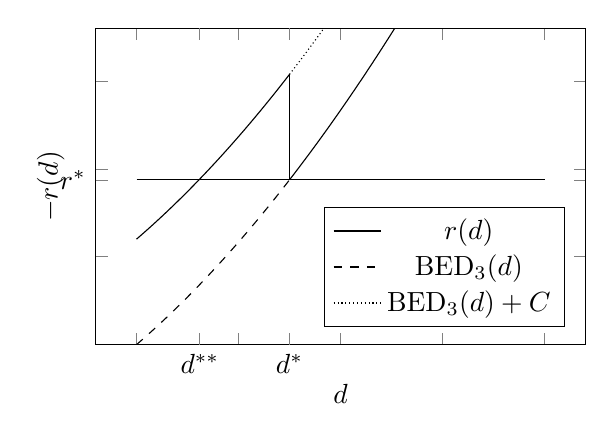
\begin{tikzpicture}
    \begin{axis}
    [
        ymin=0,
        ymax=1.8,
        xlabel={$d$}, 
        ylabel={$-r(d)$},
        ylabel style=
        {
        yshift=-3mm
        },
        xlabel style=
        {
        yshift=+1mm
        },
        yticklabels={,,},
        xticklabels={,,},
%        ticks=none,
        legend style={at={(axis cs:2.1,0.1)}, anchor=south east},
        width=7.8cm,
        height=5.6cm,
        extra y ticks={0.9375},
        extra y tick labels={$r^{*}$},
        extra x ticks={0.31, 0.75},
        extra x tick labels={$d^{**}$, $d^{*}$}
    ]
    
    \addplot[no marks, solid, domain=0:0.75, samples=50] {x + ((x^2)/3) + 0.6};
    \addlegendentry{$r(d)$}
    
    \addplot[no marks, dashed, domain=0:0.75, samples=50] {x + ((x^2)/3)};
    \addlegendentry{BED$_3(d)$}
    
    \addplot[no marks, densely dotted, domain=0.75:2, samples=50] {x + ((x^2)/3) + 0.6};
    \addlegendentry{BED$_3(d) + C$}
    
    \addplot[no marks, solid, domain=0.75:2, samples=50] {x + ((x^2)/3)};
    
    \addplot[no marks, solid, domain=0:2, samples=50] {x*0 + 0.9375};
    
    \addplot [no marks, solid, domain=0:1, samples=50]
        coordinates {(0.75,0.9375)(0.75,1.5375)};
    
    \end{axis}
\end{tikzpicture}
\caption{Qualitative description of reward function by composing negative immediate reward from BED$_{3}$ without penalty $C$ and BED$_{3}$ with penalty term $C$.}
\end{figure}

A characteristic of the specified MDP model is that the cumulative BED delivered to the OAR is not part of the state $s$. It is only integrated in the reward $r_t$ as a penalty. The reason being, that the optimal policy does not depend on the OAR state, i.e. the optimal dose to deliver does not depend on the previously accumulated BED in the OAR. Intuitively it is aimed to minimise future OAR BED, in each state and fraction, independently of the previously accumulated BED in the OAR. However, if the goal was to escalated tumor dose while delivering a fixed OAR BED, the cumulative OAR BED would be part of the state.

\paragraph{Environment Model:} The model of the environment provides the probability of    arriving in state $s_{t+1} = (\delta_{t+1}, B^T_{t})$ with reward $r_t$, starting from state $s_t$ and choosing action $d_t$. Arriving at the cumulative tumor BED $B^T_{t}$ is deterministic, as it is dependent on the previous delivered tumor BED plus action $d_t$. Arriving at the sparing factor $\delta_{t+1}$ however is a stochastic process, where $\delta$ is assumed to be normal distributed. Establishing an assumption of the environment model, completely characterises the dynamics of the Markov Process.

\subsubsection{Reward Construction}
??be more clear about rational?? Achieved should be an adaptive fractionation model that accurately steers the expected number of fractions necessary to attain a prescription tumor BED for a treatment. To determine the optimal parameter $C$ a discrete optimisation problem is formulated. To that end a penalty in the form of Eq.~\eqref{eq:penalty} with $C=0$, prescription dose $B_{\text{pres}}^{\text{T}}$ and expected probability distribution $P(\delta)$ is set. Defining a treatment for $n$ number of fractions, calculating the Bellmann Equations with these stipulations and applying the optimal policy to a set of sparing factors $\{\delta_\tau\}_{\tau=1}^{n}$, yields terminal cumulative BED $B^{\text{N}}_n$. Repeating this process by sampling sets of $\{\delta_\tau\}_{\tau=1}^{n}$ and averaging $B^{\text{N}}_n$ yields an estimate of the average terminal accumulated BED in the OAR written as $\bar{B}^{\text{N}}_n$. This is interpreted as a cost function, seeked to be minimal. In Fig.~\ref{fig:treat_policy_sigma} the qualitative example with terminal cumulative BED's $B^{\text{N}}_n$ can be seen.

To finishing the treatment with prescribed number of fraction $n_{\text{pres}}$ the reward function is constructed with a penalty parameter. The penalty parameter is given by $C$ and penalises each additional fraction  that is used for the treatment. The cost can thus be extended by linearly adding $C$ for every fraction $n$ to $\bar{B}^{\text{N}}_n$ which yields the total cost function
\begin{equation*}
    B_n = C \cdot n + \bar{B}^{\text{N}}_n
\end{equation*}
where the numeric value for $C$ can be then evaluated as minimising an objective function dependent on the minimum of $B_n$
\begin{equation*}
    C = \underset{c}{\operatorname{argmin}}\left| n_{\text{pres}} - \underset{n}{\operatorname{argmin}} \left[B_n \right] \right|
\end{equation*}
The penalty parameter $C$ can be viewed as a marginal cost with units BED per fraction. Additional fractions are used, so long that reduction of $B^{\text{N}}$ is larger than $C$. Finding the optimal parameter $C$ for a fraction using $n_{\text{pres}}$ number of fraction following equation must be fulfilled
\begin{equation*}
    \bar{B}^{\text{N}}_{n_{\text{pres}}} - \bar{B}^{\text{N}}_{n_{\text{pres}}+1} \geq C
\end{equation*}

\subsubsection{Fractionation Decision}
To translate the problem into a continuous optimisation problem, the average terminal cumulative BED $\bar{B}^{\text{N}}_n$ will be modeled according to optimal fractionation decision-making. To minimise cumulative OAR BED $B^{\text{N}}_n$ for a fixed fraction size $d_{\tau}$ and constant sparing factor with respect to the number of fractions $n$
\begin{equation*}
    \underset{n}{\text{min}} \left[ B^{\text{N}}_n \right] = \underset{n}{\text{min}} \left[ n \delta_\tau d_\tau( 1 +\frac{\delta_\tau d_\tau}{({\alpha}/{\beta})_\text{N}}) \right]
\end{equation*}
subject to tumor dose prescription
\begin{equation*}
    B^{\text{T}}_n = n d_\tau( 1 +\frac{d_\tau}{({\alpha}/{\beta})_\text{T}})
\end{equation*}
yields
\begin{equation*}
    B^{\text{N}}_n = \delta^2 n d_T(n) \left[ \frac{1}{\delta} - \frac{(\alpha / \beta) _N}{(\alpha / \beta)_T}\right] + \delta^2 B^{\text{T}}_n \frac{(\alpha / \beta) _N}{(\alpha / \beta)_T}
\end{equation*}
Note that the function is continuous and the second term is independent on $n$. Omitting this term and switching from subscript $n$ to a continous function, the BED $\bar{B}^{\text{N}}_n$ can be fitted to
\begin{equation}
    B^{\text{N}}(n; \delta) = \delta^2 n d_T(n) \left[ \frac{1}{\delta} - \frac{(\alpha / \beta) _N}{(\alpha / \beta)_T}\right]
\end{equation}
$\delta=\mu$ to averaged $B_n$, also explain how one has derived on this??
where $d_T$ is the physical dose
\begin{equation*}
    d_T(n) = \frac{\sqrt{n (\alpha / \beta)_T (n (\alpha / \beta)_T + 4 B_{\text{pres}}^{\text{T}})} - n (\alpha / \beta)_T}{2n}
\end{equation*}
Note that now there is no subscript to $B^{\text{N}}$ as it is a continuous function. This allows for a continuous objective function to be minimised for finding $C$. In the continuous case after fitting $B^{\text{N}}(n; \delta)$, $C$ can be determined analytically
\begin{equation*}
    C_{n_{\text{pres}}} = \left.\frac{\text{d} B^{\text{N}}(n; \delta)}{\text{d} n}\right|_{n=n_{\text{pres}}}
\end{equation*}
In Fig.~\ref{fig:cost_function} for $n_{\text{pres}}=5$ prescribed number of fractions the parameter $C_5=4.36$Gy was determined.

\begin{figure}[!htb]
    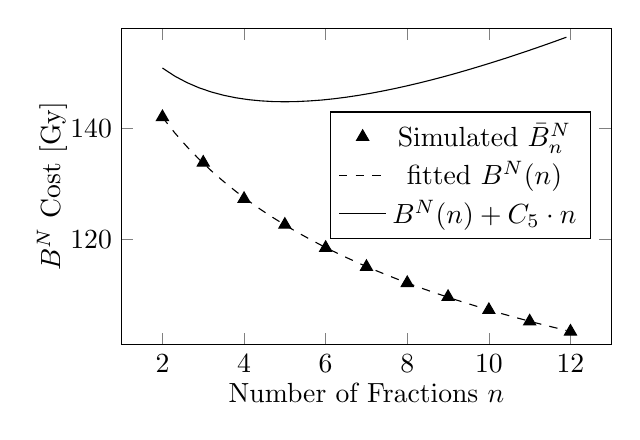
\begin{tikzpicture}
    \begin{axis}
    [
        ymin=101,
        ymax=158,
        xlabel={Number of Fractions $n$}, 
        ylabel={$B^{\text{N}}$ Cost [Gy]},
        ylabel style=
        {
        yshift=-2mm
        },
        xlabel style=
        {
        yshift=+1mm
        },
        legend style={at={(axis cs:12.5,120)}, anchor=south east},
        width=7.8cm,
        height=5.6cm
    ]  
    \addplot[only marks, mark=triangle*, mark size=2.5pt]
        coordinates {(2.0, 141.99)
            (3.0, 133.79)
            (4.0, 127.25)
            (5.0, 122.6)
            (6.0, 118.43)
            (7.0, 115.0)
            (8.0, 112.1)
            (9.0, 109.59)
            (10.0, 107.24)
            (11.0, 105.18)
            (12.0, 103.35)
        };
    \addlegendentry{Simulated $\bar{B}_n^{\text{N}}$}
    
    \addplot[no marks, dashed]
        coordinates {(2.0, 141.96)
            (2.3, 139.17)
            (2.6, 136.66)
            (2.9, 134.39)
            (3.2, 132.3)
            (3.5, 130.38)
            (3.8, 128.6)
            (4.1, 126.94)
            (4.4, 125.38)
            (4.7, 123.93)
            (5.0, 122.56)
            (5.3, 121.26)
            (5.6, 120.04)
            (5.9, 118.87)
            (6.2, 117.77)
            (6.5, 116.72)
            (6.8, 115.71)
            (7.1, 114.75)
            (7.4, 113.84)
            (7.7, 112.96)
            (8.0, 112.11)
            (8.3, 111.3)
            (8.6, 110.53)
            (8.9, 109.78)
            (9.2, 109.05)
            (9.5, 108.36)
            (9.8, 107.68)
            (10.1, 107.03)
            (10.4, 106.41)
            (10.7, 105.8)
            (11.0, 105.21)
            (11.3, 104.64)
            (11.6, 104.09)
            (11.9, 103.55)
        };
    \addlegendentry{fitted $B^{\text{N}}(n)$}
    
    \addplot[no marks, solid]
        coordinates {(2.0, 150.83)
            (2.3, 149.38)
            (2.6, 148.21)
            (2.9, 147.26)
            (3.2, 146.51)
            (3.5, 145.92)
            (3.8, 145.47)
            (4.1, 145.14)
            (4.4, 144.92)
            (4.7, 144.79)
            (5.0, 144.75)
            (5.3, 144.79)
            (5.6, 144.9)
            (5.9, 145.06)
            (6.2, 145.29)
            (6.5, 145.57)
            (6.8, 145.9)
            (7.1, 146.27)
            (7.4, 146.69)
            (7.7, 147.14)
            (8.0, 147.63)
            (8.3, 148.15)
            (8.6, 148.7)
            (8.9, 149.28)
            (9.2, 149.89)
            (9.5, 150.53)
            (9.8, 151.19)
            (10.1, 151.87)
            (10.4, 152.57)
            (10.7, 153.3)
            (11.0, 154.04)
            (11.3, 154.8)
            (11.6, 155.58)
            (11.9, 156.38)
        };
    \addlegendentry{$B^{\text{N}}(n) + C_5 \cdot n$}
    
    \end{axis}
\end{tikzpicture}
\caption{Cost function $B^{\text{N}}_n$ for a gaussian sparing factor distribution $\mu=0.9$, $\sigma=0.04$, $B_{\text{pres}}^{\text{T}}=72$. Sampled are $1000$ patients with 5 fractiona each that stem from a gaussian distribution with $\mu=0.9$, $\sigma=0.04$, $B_{\text{pres}}^{\text{T}}=72$. Values fitted with $B^{\text{N}}(n; \delta)$.}
\label{fig:cost_function}
\end{figure}
Also plotted in Fig.~\ref{fig:cost_function} is the fitting function $B^{\text{N}}(n; \delta=\mu)$ the cost is slightly higher when compared to the fit $B^{\text{N}}(n; \delta=0.89)$. Averaging the cumulative BED for $1000$ Patients each and fitting to the function $B^{\text{N}}(n;\delta)$ results in the fit parameter ($\delta$) being lower than the sparing mean $\mu=0.9$ from the sample distribution. On average Adaptive Fractionation yields slightly lower cumulative OAR BED $B^{\text{N}}$, which is reflected by a lower sparing factor as fit parameter.


\subsection{Dynamic Programming Algorithm}
\label{sec:DP}
A dynamic programming (DP) algorithm can be used to compute the optimal policy with the help of a value function \cite{sutton_reinforcement}. The value function $v_t$ describes how desirable it is to be in state $s_t$ in fraction $t$ and, therefore, it contains the information whether an action should be taken to reach that state. In this application, the value for each state represents the expected cumulative BED that can be delivered to the tumor in the remaining fractions, starting from that state and acting according to the optimal policy.

The Bellman equation relates the value function in fraction $t$ to the optimal policy and the value function in the subsequent fraction, which for this application reads
\begin{equation}\label{eq:value_function}
    \begin{split}
    v_t(\delta, & B^{\text{T}}) = \underset{d}{\text{max}} \Biggr[
    r_t(d, B^{\text{T}}) + \ldots \Biggr.\\
    & \Biggr. \sum_{\delta'}P(\delta')v_{t+1} \left( \delta', B^{\text{T}} + d + \frac{d^2}{(\alpha / \beta)_\text{T}} \right) \Biggr]
    \end{split}
\end{equation}
and the policy reads
\begin{equation}\label{eq:policy_function}
    \begin{split}
    \pi_t(\delta, & B^{\text{T}}) = \underset{d}{\text{argmax}} \Biggr[
    r_t(d, B^{\text{T}}) + \ldots \Biggr.\\
    & \Biggr. \sum_{\delta'}P(\delta')v_{t+1} \left( \delta', B^{\text{T}} + d + \frac{d^2}{(\alpha / \beta)_\text{T}} \right) \Biggr]
    \end{split}
\end{equation}
The value function $v_t(\delta, B^{\text{T}})$ is the sum of the immediate reward and the future expected reward, maximised with respect to the dose. The immediate reward consists of reward from immediate OAR BED and weighted reward from not terminating the treatment in the current fraction. The future expected reward is the future value weighted with the sparing factor probability. Abstractly speaking, the value function displays the best possible immediate and future reward summed, the algorithm can secure in each state.

In return the policy describes the optimal strategy to maximise the value function. Value function and optimal policy can be calculated iteratively in one backward recursion starting from the last fraction. To enforce the cumulative tumor BED prescription $B_{\text{pres}}^\text{T}$, a terminal reward of -$\infty$ is assigned to all terminal states in which the cumulative tumor BED prescription is not met after the last fraction. To that end, the terminal reward corresponding the value function $v_{F+1}$ at the end of the treatment after all $F$ fractions are delivered, is initialised to
\begin{equation*}
v_{F+1}(\delta_{F+1}, B^\text{T}_{F}) = 
\begin{cases}
0 & \text{if } B^\text{T}_F = B_{\text{pres}}^\text{T} \\
-\infty & \text{else}
\end{cases}
\end{equation*}

This initialises the value function and optimal policy in the last fraction $F$. Practically speaking as a consequence, optimal policy in the last fraction will simply deliver the maximum residual BED$_{10}$ to the tumor, to end up at the prescribed cumulative tumor BED given in $B_5^{\text{T}}$. Such a policy exploits above value function initialisation equation. In case prescription tumor BED cannot be achieved due to constraints in the action, the terminal reward can be initialised to a linear penalty function dependent on the difference of cumulative BED to prescription
\begin{equation*}
v_{F+1}(\delta_{F+1}, B^\text{T}_{F}) = 
- s \cdot \left| B^\text{T}_F - B_{\text{pres}}^\text{T} \right|
\end{equation*}
Where $s \gg B_{\text{pres}}^\text{T}$ is an arbitrary large number. This ensures that the policy in the last fraction is to apply the dose that minimises the difference between cumulative and prescribed BED. Policy artefacts from not reaching exactly the prescription in the last fraction due to discretisation of the actions can thus be avoided.

\subsection{Expected Remaining Number of Fractions}
It is difficult to interpret the value function with regard to the weight $C$, as the value function is composed of OAR BED rewards and reward for terminating treatment. Thus, to make the value function more interpretable, we calculated expected remaining number of fractions in the state space. The remaining number of fractions display the remaining number of fractions, that are expected in every state with. It uses the optimal policy that is already solved and the same assumptions about the probability distribution from the value function. Note that the optimal policy $\pi_t$ here is in units of BED.
\begin{equation}\label{eq:remains_function}
    \begin{split}
    \varepsilon_t(\delta, & B^{\text{T}}) =
    \eta _t (\delta, B^{\text{T}}) + \ldots \Biggr.\\
    & \Biggr. \sum_{\delta'}P(\delta') \varepsilon_{t+1} \left( \delta', B^{\text{T}} + \text{BED}_{10} \left[ \pi_t(\delta, B^{\text{T}}) \right] \right)
    \end{split}
\end{equation}
where $\eta$ is a binary function that specifies, if under the optimal policy in the current fraction the prescription dose is achieved or not.
\begin{equation}\label{eq:current_remains}
    \eta_t (\delta, B^{\text{T}}) =
    \begin{cases}
        0 & \text{if } \pi_t(\delta, B^{\text{T}}) \geq B_{\text{pres}}^{\text{T}} - B^{\text{T}} \\
        1 & \text{else}
    \end{cases}
\end{equation}
In similar manner to the value function, the terminal remaining number of fraction is initialised to
\begin{equation*}
    \varepsilon_{F+1}(\delta_{F+1}, B^\text{T}_{F}) = 0
\end{equation*}
as the in the last fraction no additional fractions are used.

\subsection{Quantification of Benefit}

The treatment plans given by Adaptive Fractionation is compared benchmarked with the following treatments

\begin{enumerate}
    \item A reference treatment in which $5 \times 8$ Gy physical dose ($14.4$ Gy BED$_{10}$, $72$ Gy $B_5^{\text{T}}$) is prescribed to the tumor in each fraction. Hence, the reference treatment delivers exactly $72$ Gy BED$_{10}$ to the tumor. It is assumed that prescribed tumor BED may be delivered to patients without compromising OAR BED constraint in the dose-limiting OAR.

%    \item An upper bound for the benefit of adaptive fractionation. To do so, we consider the hypothetical situation that all sparing factors $delta_{\tau}$ are known before treatment. In that case, the optimal doses per fraction d t is calculated by solving the following optimisation problem:
%    \begin{equation}
%        \underset{d}{\text{min }} \sum_{\tau=1}^{F}(\delta_\tau d_\tau+\frac{\delta_\tau^2 d_\tau^2}{({\alpha}/{\beta})_\text{N}})
%    \end{equation}
%    
%    \begin{equation}
%    \text{subject to } \sum_{\tau=1}^{F}(d_\tau+\frac{d_\tau^2}{({\alpha}/{\beta})_\text{T}}) \geq B^{\text{T}}_{\text{pres}}
%    \end{equation}
%    This treatment would optimally exploit the variation in $\delta$ and can thus be used to benchmark the benefit of adaptive fractionation. However, it represents an unachievable upper bound for any realistic approach to adaptive fractionation where future sparing factors are unknown.

    % \item The clinically delivered treatment has an upper limit of $5 \times 6$ Gy physical dose ($18$ Gy BED$_{3}$, $90$ Gy $B_5^{\text{N}}$ cumulative BED on the dose-limiting OAR). The clinical treatment aims to deliver the fixed prescription dose $5 \times 8$ Gy physical dose to the tumor in each fraction and may deliver less than $14.4$ Gy BED$_{10}$, in case the BED$_{3}$ OAR constraint is compromised.
\end{enumerate}

\subsection{Code Repository}

The model described in this work was implemented into the existing codebase that can be found in the public repository \cite{adaptfx_package}. Furthermore, the codebase was rebuilt the suit a command line interface, speed up calculation and streamline logic flow. These changes and extensions are given by

\paragraph{Hardcoded Settings:} Probability distribution, states and actions are discrete. Parameters defining step sizes, upper- and lower bounds for these variables were previously hardcoded whereas now they can be chosen by the user. So the resolution of the optimal policy can be adapted to a specific problem. The user can also quickly generate plots of optimal policy, value function and expected remaining number of fractions.

\paragraph{Interpolation:} It is possible that the optimal policy for reducing number of fraction is discontinuous, as for some states the remaining dose will be delivered. Discretisation of the states and actions led to artefacts (see Fig.~\ref{fig:treat_policy_c_arte}) in the discontinuous policy. The solution was to introduce linearly sampled BED action space and converting to physical dose. This allows to waive the use of interpolation. This also presumes that the stepsize for state and action have to be the same. In case they are not the same, e.g. the user wants to save computation time and set a state space lower than action space, the interpolation is used automatically.

\paragraph{Redundancy:} Multiple basic functions exist for different types to calculate the optimal policy. Instead of basic functions utilising sharing same helper functions and treatment functions the whole workflow was duplicated for each type. Every type used its own set of helper-, basic- and treatment functions which were essentially duplicates of each other. Duplicates of helper functions were made redundant and a package was streamlined that shared helper functions amongst basic functions.

\paragraph{Architecture:} The newer streamlined package offers a single treatment function that loops through the basic functions specified by the user. The user is presented with options for type of optimisation, type of probability distribution updating and options for policy calculation. All these input parameters can be specified in a dictionary inside a \texttt{python} script or a \texttt{json} file.

\paragraph{Command Line Interface:} To utilise the package in the command line, an executable is shipped that is invoked with the parameters in the \texttt{json} file. The user can specify whether to log output data during the calculation or plot information, settings of the action, policy etc. and keys for choosing optimisation method, objective  and constraints.

\paragraph{Parallelisation:} Previously in parts of the basic functions parallel computation for the value function was introduced. However, large components were still missing parallelisation. While streamlining the helper and basic functions, computation of the value function was parallelised, by introducing computation that fully supports vectorised matrix multiplication. Storing the future value function $v_{t+1}$ within each step of the iteration, allows to compute the current value function in parallel over all possible states. Parallelisation was also introduced for sampling and the probability distribution which before used first order loop. The run-time of the algorithm was improved by $8-16$ times compared to the previous approach. It runs in the order of $10^{-2}$ seconds (order of $10^{0}$ seconds before).

\subsection{Results Real Data}

For demonstration purposes a sparing factor sequence from real patient is used to apply the model. A patient who's sparing factors are exemplary to demonstrate the model, was chosen. The requirements are specified as: The sparing factors are large enough (between $0.8$ to $1.0$) that it represents a relevant case in which clinicians face the risk of compromising tumor BED, but sparing factors show large deviation to lower sparing factors, such that Adpative Fractionation is a promising strategy to mitigate this risk. In Tab.~\ref{tab:patient_sparing_factors} three candidates are shown that fulfill above requirements. For Adaptive Fractionation to be an advantageous strategy in this test setup, the sparing factors do not necessarily need large standard deviation. It is sufficient that only few sparing factors are exceptionally low compared to the mean, for Adaptive Fractionation to improve treatment quality. However, in clinical practice it is not possible to estimate whether one outling favourable sparing factor will appear through the course of the treatment, from only knowing the planning sparing factor. Rather one needs to estimate the variation of the sparing factor distribution, where outlying sparing factors are more likely for larger variation. For simplicity the treatment model assumes a fixed variation.

\paragraph{Treatment Model:} The treatment model is the prescription for the patient. It is composed of a defined total number of fractions that can be used $n_{\text{max}}=5$, a constant $C$ steering the desired number of fractions $n_{\text{pres}}=4$ that should be used, tumor dose prescription and an assumption of the sparing factor probability distribution. The variation is chosen in terms of standard deviation $\sigma = 0.10$ and the mean to be the planning sparing factor $\mu=\delta_0$. Planned is a treatment with five fractions with a tumor BED prescription of $72$ Gy which corresponds to a physical fraction dose of $8$ Gy delivered in $5$ fractions. For the parameter $C$ two values are chosen to show how the optimal policy behaves. First $C=0$ with no intention of reducing number of fractions, and additionally the optimal $C$ is evaluated according to the optimal reward section. The evaluated $C_4$ are $2.8, 2.0, 2.2$ for patients $3, 7, 13$ and is applied.

\begin{table}[!htb]
    \centering
    \caption{Patient candidates for adaptive fractionation. Given is the sparing factor in each fraction.}
    \begin{tabular}{c|cccccc}
    \toprule
        Patient & $t=$ $0$ & $1$ & $2$ & $3$ & $4$ & $5$\\
    \midrule
       3    &  $0.72$ & $0.79$ &  $0.61$ & $0.83$ & $0.77$ & $0.78$\\
       7    &  $0.64$ & $0.66$ &  $0.69$ & $0.86$ & $0.66$ & $0.57$ \\
       13   &  $0.84$ & $0.86$ &  $0.95$ & $0.88$ & $0.92$ & $0.84$ \\
     
    \bottomrule
    \end{tabular}
    \label{tab:patient_sparing_factors}
\end{table}

\begin{figure}[!htb]
    \centering
    \includegraphics[width=1\linewidth]{graphics/treat_patient_3.pdf}
    \caption{Adaptive fractionated therapy for a 5 fraction treatment applied to patient $3$. Normal distribution is estimated from planning sparing factor $\mu=\delta_0=0.72$ and fixed $\sigma=0.1$.}
    \label{fig:treat_patient_3}
\end{figure}

\begin{figure}[!htb]
    \centering
    \includegraphics[width=1\linewidth]{graphics/treat_patient_7.pdf}
    \caption{Adaptive fractionated therapy for a 5 fraction treatment applied to patient $7$. Normal distribution is estimated from the planning sparing factor $\mu=\delta_0=0.64$, $\sigma=0.1$.}
    \label{fig:treat_patient_7}
\end{figure}

\begin{figure}[!htb]
    \centering
    \includegraphics[width=1\linewidth]{graphics/treat_patient_13.pdf}
    \caption{Adaptive fractionated therapy for a 5 fraction treatment applied to patient $13$. Normal distribution is estimated from the planning sparing factor $\mu=\delta_0=0.84$, $\sigma=0.1$.}
    \label{fig:treat_patient_13}
\end{figure}

\begin{table}[!htb]
    \centering
    \caption{Comparison of accumulated OAR BED $B_5^{\text{N}}$ for Uniform Fractionation (UF) and Adaptive Fractionation (AF). The number of fraction used to complete the tumor prescription dose of $72$ Gy is given by $n_{\text{frac}}$.}
    \begin{tabular}{cl|cc}
    \toprule
        Patient & Fractionation & $B_5^{\text{N}}$ [Gy] & $n_{\text{frac}}$ \\
    \midrule
        3  & UF         & $91.8$ & 5 \\
           & AF $C=0$   & $75.1$ & 5 \\
           & AF $C=2.8$ & $75.6$ & 2 \\
    \midrule
        7  & UF         & $79.0$ & 5 \\
           & AF $C=0$   & $76.2$ & 5 \\
           & AF $C=2.0$ & $79.5$ & 4 \\
    \midrule
        13 & UF        & $120.3$ & 5 \\
          & AF $C=0$   & $123.1$ & 5 \\
          & AF $C=2.2$ & $123.1$ & 5 \\
     
    \bottomrule
    \end{tabular}
    \label{tab:result_treat_patient}
\end{table}

\subsection{Results Synthetic Data}

We introduce a synthetic patient is introduced to further demonstrate the model on a sequence of sparing factors. The synthetic patient is a patient not based on real data, but manually specified data. The sparing factors of the synthetic patient are chosen such, that the patient represents a relevant case in which the prescribed tumor BED may be compromised. In this section we will look at the accumulated BED results, when applying the strategies of adaptive fractionation to the synthetic patient. Hence, an according treatment model is composed, that defines prescription to the patient. Demonstrations based on the synthetic patient and treatment model include: calculation of the optimal policy and retrospective application of this policy to the synthetic patient.

\paragraph{Treatment Model:} The treatment model is planned with $n_{\text{max}}=5$ and $4$ desired number of fractions $n_{\text{pres}}=4$. Planned is the same treatment as with the real patient data, with a tumor BED prescription of $72$ Gy which corresponds to a physical fraction dose of $8$ Gy delivered in $5$ fractions. For the parameter $C$ two values ($0, 1,2$) are chosen to show how the optimal policy behaves. In addition, the optimal $C$ is evaluated according to the optimal reward section. The evaluated $C_4$ is $3.0$ and is applied. The sparing factor probability distribution is assumed to be normal distributed with mean $\mu=0.75$ and standard deviation $\sigma = 0.10$. A sequence of sparing factors close to $0.75$ in every fraction, corresponds to the clinical case, where the tumor dose may be compromised due to the risk of violating OAR dose constraint.

\paragraph{Patient Model:} In this cas the patient model describes a manually chosen sequence of sparing factors for the synthetic patient. Through the retrospective treatment observed sparing factors of this synthetic patient are $\{\delta_\tau\}_{\tau=1}^{t=5} = \{\mu, \mu \pm \sigma, \mu,\mu, \mu \}$. In the second fraction a deviation from the mean sparing factor will appear to demonstrate the applied policy. Note the first sparing factor in fraction $\tau=0$ is the planning sparing factor and not sampled here, as it is not used.

\begin{figure}[!htb]
    \centering
    \includegraphics[width=1\linewidth]{graphics/treat_patient_synthetic.pdf}
    \caption{Adaptive fractionated therapy for a 5 fraction treatment with assumed normal distribution $\mu=0.75$, $\sigma=0.1$. Synthetic patient has a sparing factor in the second fraction, which is a standard deviation lower than the mean.}
    \label{fig:treat_patient_synthetic}
\end{figure}

The constructed synthetic patient has sparing factor sequence of $0.75$ for all fractions except in the second fraction $\delta_2 = 0.65$.  Applying the treatment model to the synthetic patient, the cumulative BED $B_5^{\text{N}}$ for $C=0$ results in $80.8$ Gy. Comparing this to uniform fractionation (delivering $8$ Gy physical dose to the tumor in each fraction) yields a BED$_3$ of $18$ Gy for each fraction with $\delta=0.75$ and a BED$_3$ of $14.21$ Gy for $\delta_2=0.65$, resulting in $86.21$ Gy cumulative BED $B_5^{\text{N}}$. Thus, Adaptive Fractionation for this specific patient and treatment model surpasses OAR sparing by delivering $5.41$ Gy less cumulative BED $B_5^{\text{N}}$ compared to uniform fractionation. Applying Adaptive Fractionation with $C=1.2$ and $C=1.3$ results in the treatment terminating with $4$ respectively $2$ fractions (see Fig.~\ref{fig:treat_patient_synthetic}) while still delivering less cumulative BED $B_5^{\text{N}}$ than uniform fractionation and reaching prescribed tumor dose of $72$ Gy. In Tab.~\ref{tab:result_treat_fraction_4} the comparison is summarised.

\begin{table}[!htb]
    \centering
    \caption{Comparison of accumulated OAR BED $B_5^{\text{N}}$ for Uniform Fractionation (UF) and Adaptive Fractionation (AF). The number of fraction used to complete the tumor prescription dose of $72$ Gy is given by $n_{\text{frac}}$. Sparing factors are $\delta_t=0.75$ except for $\delta_2=0.65$}
    \begin{tabular}{cl|cc}
    \toprule
        Patient & Fractionation & $B_5^{\text{N}}$ [Gy] & $n_{\text{frac}}$ \\
    \midrule
        Synthetic   & UF &  $86.2$ & 5 \\
                    & AF $C=0$ & $80.8$ & 5 \\
                    & AF $C=1.2$ & $82.0$ & 4 \\
                    & AF $C=1.3$ & $83.8$ & 2 \\
     
    \bottomrule
    \end{tabular}
    \label{tab:result_treat_fraction_4}
\end{table}

Presented are the corresponding value functions. To interpret the results the policy as well as the expected remaining number of fractions for the treatment model are shown.

\begin{figure}[!htb]
    \centering
    \includegraphics[width=1\linewidth]{graphics/treat_values.pdf}
    \caption{Value function for a 5 fraction treatment with assumed normal distribution $\mu=0.75$, $\sigma=0.1$ and $C=0$.}
    \label{fig:treat_values}
\end{figure}

\begin{figure}[!htb]
    \centering
    \includegraphics[width=1\linewidth]{graphics/treat_values_single.pdf}
    \caption{Value function in the last fraction for a 5 fraction treatment with assumed normal distribution $\mu=0.75$, $\sigma=0.1$ and arbitrary $C=0$.}
    \label{fig:treat_values_single}
\end{figure}

\begin{figure}[!htb]
    \centering
    \includegraphics[width=1\linewidth]{graphics/treat_values.pdf}
    \caption{Value function for a 5 fraction treatment with assumed normal distribution $\mu=0.75$, $\sigma=0.1$ and $C=1.2$.}
    \label{fig:treat_values_c}
\end{figure}

\begin{figure}[!htb]
    \centering
    \includegraphics[width=1\linewidth]{graphics/treat_values_single.pdf}
    \caption{Value function in the last fraction for a 5 fraction treatment with assumed normal distribution $\mu=0.75$, $\sigma=0.1$ and arbitrary $C=1.2$.}
    \label{fig:treat_values_single_c}
\end{figure}

Optimal policy for the treatment model with $\sigma=0.1$ and $C=0$ applied for the synthetic patient can be seen in Fig.~\ref{fig:treat_policy} and Fig.~\ref{fig:treat_policy_single}.

\begin{figure}[!htb]
    \centering
    \includegraphics[width=1\linewidth]{graphics/treat_policy.pdf}
    \caption{Optimal policy for a 5 fraction treatment with assumed normal distribution $\mu=0.75$, $\sigma=0.1$ and $C=0$. Policy of the last fraction is not shown as it applies the remaining dose regardless of the sparing factor.}
    \label{fig:treat_policy}
\end{figure}

For parameter $C=1.2$ the optimal policy is displayed in Fig.~\ref{fig:treat_policy_c} and Fig.~\ref{fig:treat_policy_single}. In each fraction there is one plateau at in each policy function. Landing on such a plateau in the state space, means the optimal policy is to deliver the remaining dose to finish the treatment in the current fraction.

\begin{figure}[!htb]
    \centering
    \includegraphics[width=1\linewidth]{graphics/treat_policy_c.pdf}
    \caption{Optimal policy for a 5 fraction treatment with assumed normal distribution $\mu=0.75$, $\sigma=0.1$ and $C=1.2$. Policy of the last fraction is not shown as it applies the remaining dose regardless of the sparing factor.}
    \label{fig:treat_policy_c}
\end{figure}

For the case in which $C=0$ and $\sigma=0.1$ in the expected remaining number of fractions Fig.~\ref{fig:treat_remains_c} appears one and very narrow plateau on the bottom for states close to the prescribed tumor dose. This plateau corresponds to the states where the optimal policy will finish the treatment in the current fraction. Realistically this plateau will not be reached if the optimal dose in the previous fraction is delivered.

\begin{figure}[!htb]
    \centering
    \includegraphics[width=1\linewidth]{graphics/treat_remains.pdf}
    \caption{Expected remaining number of fractions for a 5 fraction treatment with assumed normal distribution $\mu=0.75$, $\sigma=0.1$ and $C=0$. Last fraction is not shown as it is zero for every state.}
    \label{fig:treat_remains}
\end{figure}

In Fig.~\ref{fig:treat_remains_c} the case $C=1.2$, $\sigma=0.1$ is displayed. Compared to Fig.~\ref{fig:treat_remains} the plateau in each fraction spans through nearly all the accumulated dose states $B^{\text{T}}$. And compared to Fig.~\ref{fig:treat_remains_c_plat} no plateau steps but rather a pronounced gradient to larger expected remaining number of fractions appear. In fraction $t=4$ the expected remaining number is binary, as the treatment either finishes in the current fraction $t=4$ or one additional fraction will be used, such that the treatment is finished in fraction $t=5$.

\begin{figure}[!htb]
    \centering
    \includegraphics[width=1\linewidth]{graphics/treat_remains_c.pdf}
    \caption{Expected remaining number of fractions for a 5 fraction treatment with assumed normal distribution $\mu=0.75$, $\sigma=0.1$ and $C=1.2$. Last fraction is not shown as it is zero for every state.}
    \label{fig:treat_remains_c}
\end{figure}

\section{Patient Data and Treatment Plans}

Considered are patients with abdominal tumors in proximity to either bowel, stomach or duodenum and prostate cancer in proximity to the rectum. For prostate cases urethra and bladder are ignored. These patients received 5-fraction SBRT treatments at the MR-Linac system (MRIdian, Viewray). All patients were planned and treated according to institutional practice. In addition to the simulation MR and CT scans, daily MR scans were performed for on-line adaptive radiotherapy. Tumors and OARs in a $2$cm ring around the tumor were recontoured according to institutional guidelines and daily adaptive treatment plans were created. In each fraction the dose distributions were reoptimised, to adapt to inter-fractional changes, without altering the prescription dose.

\subsection{Motivation}
Thus far we described and demonstrated the optimal policy with exemplary synthetic patients (sparing factors). In a next step the goal was to find a target in clinical practice which is suitable for applying the model. A prospective candidate target ideally shows large expected variation in sparing factors. We decided to also look at correlation between spatial distance in target-OAR pair and sparing factor to see if one can intuitively guess the quality of the sparing factor.


\subsection{Methods}
Patient data was collected manually from the treatment planning system to get an overview of the distance between OAR and tumor volumes in relation to sparing factor. In total $30$ patients were extracted from the treatment planning system, $10$ for each target. In case of the prostate target $5$ patients with CTV as volume of interest and $5$ patients with boost target volume as volume of interest were collected. Boost target volumes were collected for patients treated with simultaneous integrated boost strategy \cite{orlandi_sib_clinical} \cite{mohan_sib}. For each patient also extracted were the following variables:

\paragraph{Target:} $10$ patients were extracted for each tumor that was either pancreas, adrenal glands or prostate cancer. Depending on the predictor the volume for the target was defined for either GTV, PTV, CTV or DIL the volume for prostate boost volume.

\paragraph{OAR:} For each patient at least one of the OAR in proximity was extracted. There were two criteria which qualified an OAR to be registered. The first was if the OAR was dose-limiting and the second if the OAR was in close vicinity: Every OAR in one patient that was as close to the tumor as the dose-limiting OAR in at least one fraction, was tracked as well. Only patients were collected, where the dose-limiting OAR did not change during the treatment.

% \paragraph{Overlap Status:} The overlap was chosen as predictor whether the distance $w$ will be small between target and OAR. In the treatment planning system it was checked if in one of the sagittal, transversal or coronal plane there was an overlap between the target volume and OAR.

\paragraph{Distance:} Distance between target and OAR was the shortest measured distance in all the sagittal, transversal or coronal plane. In principle no overlap was allowed between GTV and OAR. However, if there was an overlap the furthest radial distance of the overlap was measured.

\paragraph{OAR/Target Dose:} For pancreas and adrenal glands dose to OAR $d^{\text{N}}$ and dose to target $d$ were measured according to the definition in Sec.~\ref{sec:sparing_factors}. For prostate the parameter definition was different and can be found in Tab.~\ref{tab:operational_quantity} alongside pancreas and adrenal glands parameter definition. The predictors were directly extracted from the DVH in physical dose calculated in the treatment planning system.

A table with which operational quantities for each target were chosen as predictors can be seen in Tab.~\ref{tab:operational_quantity}. The predictors were extracted for each tumor-OAR pair for $6$ treatment plans in each patient, corresponding to the $5$ delivered plans and the initial plan based on the planning MR.

\begin{table}[!htb]
    \centering
    \caption{Operational quantities collected at the MR-Linac. Explained are target dose definition and volume. Targets are PAN (pancreas), ADN (adrenal glands), prostate (PRO) and BST (prostate boost volume)}
    \begin{tabular}{l|lll}
    % \toprule
    %     Target & Overlap & $w$ & $d^{\text{N}}$ [Gy] & $d$ [Gy] \\
    % \midrule
    %    PAN & PTV & GTV & $D_{1\text{cc}}$   & $D_{95}$ PTV \\
    %    ADN & PTV & GTV & $D_{1\text{cc}}$   & $D_{95}$ PTV \\
    %    PRO & PTV & CTV & $D_{1\text{cc}}$   & $D_{95}$ PTV \\
    %    BST & DIL & DIL & $D_{0.1\text{cc}}$ & $D_{95}$ DIL \\
    \toprule
        Target & $w$ & $d^{\text{N}}$ [Gy] & $d$ [Gy] \\
    \midrule
       PAN & GTV & $D_{1\text{cc}}$   & $D_{95}$ PTV \\
       ADN & GTV & $D_{1\text{cc}}$   & $D_{95}$ PTV \\
       PRO & CTV & $D_{1\text{cc}}$   & $D_{95}$ PTV \\
       BST & DIL & $D_{0.1\text{cc}}$ & $D_{95}$ DIL \\
     
    \bottomrule
    \end{tabular}
    \label{tab:operational_quantity}
\end{table}

\subsection{Patient Data}

\subsubsection{Pancreas Patients}

Sparing factors dependent on spatial distance between target-OAR pair are shown in Fig.~\ref{fig:data_pan_0} for pancreas patients. Sparing factors that were near $1.1$ also showed overlap in GTV and OAR. An example of such overlap would be patient $1$ for whom sparing factors both with duodenum and stomach are distributed around $1.0$ and distance between $0.0$ to $-0.3$ cm. Note that for patient $1$ the stomach was the dose-limiting OAR. Information of sparing factors grouped by patients are shown in Fig.~\ref{fig:data_pan_1}. Other notable cases are patient $6$ and $8$ which show only dose-limiting OAR with almost no variation in distance. Patient sparing factors are always closely clustered together. This close clustering for each patient is also visible in Fig.~\ref{fig:data_pan_2}, where sparing factors are grouped only by patients without spatial distance. Sparing factors in dose-limiting OAR range from $0.56$ to $1.1$. Displayed in Fig.~\ref{fig:data_pan_3}, is the temporal course of the sparing factors and spatial distances. Tendency is that sparing factor is lower if distance is larger, however not always the case. When looking at patients $6$ and $8$ where distances are similar, the sparing factor ranges from $1.0$ to $1.1$ for patient $6$ and $0.85$ to $1.0$ for patient $8$.

\begin{figure}[!htb]
    \centering
    \includegraphics[width=1\linewidth]{graphics/data_pan_0.pdf}
    \caption{10 pancreas patients treated at the MR-Linac. Sparing factors $\delta$ dependent on distance $w$ grouped by OAR. Multiple OAR were collected per patient and not only the dose-limiting OAR.}
    \label{fig:data_pan_0}
\end{figure}

\begin{figure}[!htb]
    \centering
    \includegraphics[width=1\linewidth]{graphics/data_pan_1.pdf}
    
    \caption{10 pancreas patients treated at the MR-Linac. Sparing factors $\delta$ dependent on distance $w$ grouped by patient. Row shows all collected OAR per patient.}
    \label{fig:data_pan_1}
\end{figure}

\begin{figure}[!htb]
    \centering
    \includegraphics[width=1\linewidth]{graphics/data_pan_2.pdf}
    \caption{10 pancreas patients treated at the MR-Linac. Sparing factors $\delta$ for each patient grouped by dose-limiting OAR.}
    \label{fig:data_pan_2}
\end{figure}

\begin{figure}[!htb]
    \centering
    \includegraphics[width=1\linewidth]{graphics/data_pan_3.pdf}
    \caption{10 pancreas patients treated at the MR-Linac. Sparing factors $\delta$ (shown as triangles) and distance $w$ (shown as lines) displayed for each fraction grouped by patient. Row shows dose-limiting OAR.}
    \label{fig:data_pan_3}
\end{figure}

\subsubsection{Adrenal Glands Patients}

Sparing factors dependent on spatial distance between target-OAR pair are shown in Fig.~\ref{fig:data_adn_0} for adrenal glands patients. There are no sparing factors that are larger than $1$ and also no overlaps registered in GTV and OAR. Fig.~\ref{fig:data_adn_1} displays the same picture as Fig.~\ref{fig:data_pan_1} but this time additionally grouped by patients. Important to note is that sparing factors range from $0.2$ to $1.0$ in stomach and  $0.05$ to $1.0$ in bowel. Sparing factors per patient are closely clustered together but across the cohort shows a much wider spread of the variation in sparing factors. Looking at the sparing factors for each patient and only dose-limiting OAR in Fig.~\ref{fig:data_adn_2}, it is also visible that they are closer clustered together for each patient compared to Fig.~\ref{fig:data_pan_2}. Sparing factors in dose-limiting OAR range from $0.2$ to $1.0$. Displayed in Fig.~\ref{fig:data_pan_3}, is the temporal course of the sparing factors and spatial distances. Tendency is that sparing factor is lower if distance is larger, however not always the case. When looking at patients $6$ and $8$ where distances are similar, the sparing factor ranges from $1.0$ to $1.1$ respectively $0.85$ to $1.0$.


\begin{figure}[!htb]
    \centering
    \includegraphics[width=1\linewidth]{graphics/data_adn_0.pdf}
    \caption{10 adrenal gland patients treated at the MR-Linac. Sparing factors $\delta$ dependent on distance $w$ grouped by OAR. Multiple OAR were collected per patient and not only the dose-limiting OAR.}
    \label{fig:data_adn_0}
\end{figure}

\begin{figure}[!htb]
    \centering
    \includegraphics[width=1\linewidth]{graphics/data_adn_1.pdf}
    \caption{10 adrenal gland patients treated at the MR-Linac. Sparing factors $\delta$ dependent on distance $w$ grouped by patient. Row shows all collected OAR per patient.}
    \label{fig:data_adn_1}
\end{figure}

\begin{figure}[!htb]
    \centering
    \includegraphics[width=1\linewidth]{graphics/data_adn_2.pdf}
    \caption{10 adrenal gland patients treated at the MR-Linac. Sparing factors $\delta$ for each patient grouped by dose-limiting OAR.}
    \label{fig:data_adn_2}
\end{figure}

\begin{figure}[!htb]
    \centering
    \includegraphics[width=1\linewidth]{graphics/data_adn_3.pdf}
    \caption{10 adrenal gland patients treated at the MR-Linac. Sparing factors $\delta$ (shown as triangles) and distance $w$ shown (as lines) displayed for each fraction grouped by patient. Row shows dose-limiting OAR.}
    \label{fig:data_adn_3}
\end{figure}

\subsubsection{Prostate Patients}

Prostate cases are not grouped by OAR but rather specific target volume, since the OAR registered was only rectum. There is no variation in spatial distance when looking at prostate CTV in Fig.~\ref{fig:data_pro_0}. The volumes always touched but did not overlap in any fraction. Fig.~\ref{fig:data_pro_1} and Fig.~\ref{fig:data_pro_2} shows sparing factors ranging between $0.97$ to $1.06$ for prostate CTV and $0.89$ to $0.97$ for boost volume which is lower. Sparing factors between the two target volumes are overall similar in variation, however Fig.~\ref{fig:data_pro_1} displays larger variation in spatial distance in boost volume compared to prostate CTV. In Fig.~\ref{fig:data_pro_3} it is well visible that there is no variation in spatial distance for each patient, when looking at patients with prostate CTV registered.

\begin{figure}[!htb]
    \centering
    \includegraphics[width=1\linewidth]{graphics/data_pro_0.pdf}
    \caption{10 prostate patients treated at the MR-Linac. Sparing factors $\delta$ dependent on distance $w$ grouped by target volume BST (prostate boost volume) and PRO (prostate CTV).}
    \label{fig:data_pro_0}
\end{figure}

\begin{figure}[!htb]
    \centering
    \includegraphics[width=1\linewidth]{graphics/data_pro_1.pdf}
    \caption{10 prostate patients treated at the MR-Linac. Sparing factors $\delta$ dependent on distance $w$ grouped by target volume BST (prostate boost volume) and PRO (prostate CTV).}
    \label{fig:data_pro_1}
\end{figure}

The sparing factors of the integrated boost volume are misleading. Dose to the tumor for large distances between rectum and boost volume, was not escalated. Instead, clinicians prescribed and delivered a $D_{95}$ of $40$ Gy physical dose in every fraction. For patients $27$ and $28$ the distance is very large with distance around $1$ respectively $1.5$cm. In regard to the sparing factor the dose could theoretically have been escalated even further than prescribed $D_{95}$ of $40$ Gy physical dose.

\begin{figure}[!htb]
    \centering
    \includegraphics[width=1\linewidth]{graphics/data_pro_2.pdf}
    \caption{10 prostate patients treated at the MR-Linac. Sparing factors for each patient grouped by target volume BST (prostate boost volume) and PRO (prostate CTV).}
    \label{fig:data_pro_2}
\end{figure}

\begin{figure}[!htb]
    \centering
    \includegraphics[width=1\linewidth]{graphics/data_pro_3.pdf}
    \caption{10 prostate patients treated at the MR-Linac. Sparing factors $\delta$ (shown as triangles) and distance $w$ (shown as lines) displayed for each fraction grouped by target volume BST (prostate boost volume) and PRO (prostate CTV)}
    \label{fig:data_pro_3}
\end{figure}

\section{Discussion}

- no patients from prostate suitable
- misleading sparing factor BST
- few patients in adrenal glands suitable



\clearpage
\newpage

\printbibliography{}

\newpage

\section*{Appendix}

\addcontentsline{toc}{section}{\protect\numberline{}Appendix}%


\renewcommand{\thesubsection}{\Alph{subsection}}
\renewcommand\thefigure{\thesubsection.\arabic{figure}}

\setcounter{figure}{0}
\setcounter{subsection}{0}

%----------------------------------------------

\subsection{Other Notable Results}

Described and illustrated are the other treatment model regarding policy, value function and expected remaining number of fractions.

\subsubsection{Treatment Model}

For the parameter $C$ multiple values are chosen to show how the optimal policy behaves. The sparing factor probability distribution is assumed to be normal distributed with mean $\mu=0.75$ and standard deviation $\sigma = \{ 0.001, 0.05, 0.10, 0.15\}$. A sequence of sparing factors close to $0.75$ in every fraction, corresponds to the clinically interesting case, where the tumor dose may be compromised due to the risk of violating OAR dose constraint. Provided enough variation in such a case Adaptive Fractionation could bring a benefit to patients, by reducing cumulative dose to OAR.

\subsubsection{Policy}

The optimal policy $\pi_t(\delta, B^{\text{T}})$ for a 5 fraction treatment with normal distribution $\mu=0.75$ and very low standard variation of $\sigma=0.001$ is given in Fig.~\ref{fig:treat_policy_sigma} and Fig.~\ref{fig:treat_policy_single}. The probability distribution $P(\delta)$ is fixed: i.e. the optimal policy for the entire treatment is solved without updating the probability distribution with progressing treatment.

\begin{figure}[!htb]
    \centering
    \includegraphics[width=1\linewidth]{graphics/treat_policy_sigma.pdf}
    \caption{Optimal policy for a 5 fraction treatment with assumed normal distribution $\mu=0.75$, $\sigma=0.001$ and $C=0$. Policy of the last fraction is not shown as it applies the remaining dose regardless of the sparing factor.}
    \label{fig:treat_policy_sigma}
\end{figure}

For the same expected probability distribution but increasing $C$ gives the policy seen in Fig.~\ref{fig:treat_policy_c_plat} and~\ref{fig:treat_policy_single}. A feature of this policy is the appearance of plateaux and thus a discontinuous policy function.

\begin{figure}[!htb]
    \centering
    \includegraphics[width=1\linewidth]{graphics/treat_policy_c_plat.pdf}
    \caption{Optimal policy for a 5 fraction treatment with assumed normal distribution $\mu=0.75$, $\sigma=0.001$ and $C=1.9$. Policy of the last fraction is not shown as it applies the remaining dose regardless of the sparing factor.}
    \label{fig:treat_policy_c_plat}
\end{figure}

\begin{figure}[!htb]
    \centering
    \includegraphics[width=1\linewidth]{graphics/treat_policy_single.pdf}
    \caption{Optimal policy in the last fraction for an arbitrary 5 fraction treatment. Policy in the last fraction applies the remaining dose regardless of the sparing factor.}
    \label{fig:treat_policy_single}
\end{figure}

\begin{figure}[!htb]
    \centering
    \includegraphics[width=1\linewidth]{graphics/treat_policy_c_arte.pdf}
    \caption{Optimal policy for a 5 fraction treatment with assumed normal distribution $\mu=0.75$, $\sigma=0.1$ and $C=1.2$, polluted with artefacts due to interpolation.}
    \label{fig:treat_policy_c_arte}
\end{figure}

\begin{figure}[!htb]
    \centering
    \includegraphics[width=1\linewidth]{graphics/treat_values_c_plat.pdf}
    \caption{Value function for a 5 fraction treatment with assumed normal distribution $\mu=0.75$, $\sigma=0.001$ and $C=1.9$.}
    \label{fig:treat_values_c_plat}
\end{figure}

\begin{figure}[!htb]
    \centering
    \includegraphics[width=1\linewidth]{graphics/treat_values_c_plat_single.pdf}
    \caption{Value function in the last fraction for a 5 fraction treatment with assumed normal distribution $\mu=0.75$, $\sigma=0.001$ and arbitrary $C$.}
    \label{fig:treat_values_c_plat_single}
\end{figure}

\subsubsection{Expected Remaining Number of Fractions}

Since the policy is known for every state the expected remaining number of fractions can be calculated for every fraction. In Fig.~\ref{fig:treat_remains_c_plat} the remaining number of fractions are shown to the policy in Fig.~\ref{fig:treat_policy_c_plat} shown before. The bottom plateau in the policy correspond to the states where the treatment is will be finished in the current fraction. One plateau above correspond to all states where it is expected to finish treatment the next fraction. The further along in the treatment, the fewer fractions are remaining and thus plateaux disappear. The number of plateaux in a fraction is equal to the number of fractions remaining including the current fraction.

\begin{figure}[!htb]
    \centering
    \includegraphics[width=1\linewidth]{graphics/treat_remains_c_plat.pdf}
    \caption{Expected remaining number of fractions for a 5 fraction treatment with assumed normal distribution $\mu=0.75$, $\sigma=0.001$ and $C=1.9$. Last fraction is not shown as it is zero for every state.}
    \label{fig:treat_remains_c_plat}
\end{figure}

Described and illustrated are the treatment models applied to a synthetic patient with varying observed sparing factors chosen for demonstration. 

\subsubsection{Constant Sparing Factor}
If a synthetic patient shows no deviation at all with sparing factors appearing at $\mu = 0.75$. A uniformly fractionated treatment plan yields the limiting $90$ Gy cumulative OAR BED $B_5^{\text{N}}$ for a tumor prescription dose of $72$ Gy. Assuming an Adaptive Fractionation treatment model with a low variation in sparing factors, such that practically there is no variation expected at all and a constant $C=0$ (see Fig.~\ref{fig:treat_fraction_0}), the policy conforms to uniform fractionation. Increasing $C$ yields uniform fractionation policy using fewer fractions and resulting in higher $B_5^{\text{N}}$.
\begin{figure}[!htb]
    \centering
    \includegraphics[width=1\linewidth]{graphics/treat_fraction_0.pdf}
    \caption{Adaptive fractionated therapy for a 5 fraction treatment with assumed normal distribution $\mu=0.75$, $\sigma=0.001$. Sparing factor is the same for every fraction including planning.}
    \label{fig:treat_fraction_0}
\end{figure}

Increasing the expected variation in sparing factors to a standard deviation of $\sigma=0.05$ seen in Fig.~\ref{fig:treat_fraction_1} for otherwise equal treatment model, yields higher cumulative BED $B_5^{\text{N}}$ compared to a $\sigma=0.001$. For $C=0$ less dose is applied in the first three fractions compared to the treatment model with $\sigma=0.001$, as a variation in favour of lower sparing factors is expected. As no lower sparing factors appear the dose is steadily increased. Looking at the treatment model with $C=4.4$ the treatment is finished after 4 fractions with a cumulative BED $B_5^{\text{N}}$ $3.5$ Gy higher compared to uniform fractionation.

\begin{figure}[!htb]
    \centering
    \includegraphics[width=1\linewidth]{graphics/treat_fraction_1.pdf}
    \caption{Adaptive fractionated therapy for a 5 fraction treatment with assumed normal distribution $\mu=0.75$, $\sigma=0.05$. Sparing factor is the same for every fraction including planning.}
    \label{fig:treat_fraction_1}
\end{figure}

Increasing the expected variation in sparing factors even further to a standard deviation of $\sigma=0.1$ and $\sigma=0.15$ seen in Fig.~\ref{fig:treat_fraction_2} and Fig.~\ref{fig:treat_fraction_3} for otherwise equal treatment model for $C=4.4$ and $C=5.0$ parameters only one fraction is omitted.

\begin{figure}[!htb]
    \centering
    \includegraphics[width=1\linewidth]{graphics/treat_fraction_2.pdf}
    \caption{Adaptive fractionated therapy for a 5 fraction treatment with assumed normal distribution $\mu=0.75$, $\sigma=0.1$. Sparing factor is the same for every fraction including planning.}
    \label{fig:treat_fraction_2}
\end{figure}

For a patient model with zero variation in sparing factor and treatment model with large expected variation the optimal policy yields a suboptimal dose delivery reflected by the higher cumulative BED $B_5^{\text{N}}$ compared to a treatment model that assumes low variation.

\begin{figure}[!htb]
    \centering
    \includegraphics[width=1\linewidth]{graphics/treat_fraction_3.pdf}
    \caption{Adaptive fractionated therapy for a 5 fraction treatment with assumed normal distribution $\mu=0.75$, $\sigma=0.15$. Sparing factor is the same for every fraction including planning.}
    \label{fig:treat_fraction_3}
\end{figure}

\subsubsection{Deviation from the Sparing Factor}

Applying a treatment model with an expected standard deviation $\sigma=0.1$ to a patient model with a sparing factor sequence of $0.75$ for all fractions except in the second fraction $\delta_2 = 0.85$, the cumulative BED $B_5^{\text{N}}$ compared to a patient model with no variation is lower. The uniform fractionation (delivering $8$ Gy physical dose to the tumor in each fraction) yields a BED$_3$ of $18$ Gy for each fraction with sparing factor $0.75$ and a BED$_3$ of $22.21$ Gy for $\delta_2=0.85$, resulting in $94.21$ Gy. Adaptive Fractionation for 5 fraction treatment ($C=0$) surpasses OAR sparing by delivering $1.81$ Gy less cumulative BED $B_5^{\text{N}}$ compared to uniform fractionation.

Adaptive Fractionation with a treatment model of $C=1.2$ and $C=3$ do not finish the treatment earlier than 5 fractions (see Fig.~\ref{fig:treat_fraction_5}) and deliver the same cumulative BED $B_5^{\text{N}}$ as the treatment model with $C=0$. Nevertheless, the cumulative BED $B_5^{\text{N}}$ is still lower than uniform fractionation while reaching prescribed tumor dose of $72$ Gy. The optimal policy does not allow increasing dose to omit fractions, due to the exceptional high sparing factor of $0.85$. In Tab.~\ref{tab:result_treat_fraction_5} the comparison is summarised.

\begin{figure}[!htb]
    \centering
    \includegraphics[width=1\linewidth]{graphics/treat_fraction_5.pdf}
    \caption{Adaptive fractionated therapy for a 5 fraction treatment with assumed normal distribution $\mu=0.75$, $\sigma=0.1$. Sparing factor in the second fraction is a standard deviation higher from the mean.}
    \label{fig:treat_fraction_5}
\end{figure}

\begin{table}[!htb]
    \centering
    \caption{Comparison of accumulated OAR BED $B_5^{\text{N}}$ for Uniform Fractionation (UF) and Adaptive Fractionation (AF). The number of fraction used to complete the tumor prescription dose of $72$ Gy is given by $n_{\text{frac}}$. Sparing factors are $\delta_t=0.75$ except for $\delta_2=0.85$}
    \begin{tabular}{l|cc}
    \toprule
        Fractionation & $B_5^{\text{N}}$ [Gy] & $n_{\text{frac}}$ \\
    \midrule
       UF &  $94.2$ & 5 \\
       AF $C=0$ & $92.4$ & 5 \\
       AF $C=1.2$ & $92.3$ & 5 \\
       AF $C=1.3$ & $92.3$ & 5 \\
     
    \bottomrule
    \end{tabular}
    \label{tab:result_treat_fraction_5}
\end{table}

\subsection{Probability Updating}
\label{sec:probupdate}
The DP algorithm relies on a description of the environment to compute an optimal policy, in this case the probability distribution of the sparing factor $P(\delta)$, which we assume to be a Gaussian distribution truncated at $0$, with patient-specific parameters for mean and standard deviation. At the start of a treatment, only two sparing factors are available for that patient, from the planning scan and the first fraction. In each fraction, an additional sparing factor is measured, which can be used to calculate updated estimates $\mu_t$ and $\sigma_t$ for mean and standard deviation, respectively.

\subsubsection{Maximum a Posteriori Estimation}
In each fraction $t$, the maximum likelihood estimator of the mean of the sparing factor distribution is
\begin{equation}\label{eq:mean}
\mu_t = \frac{1}{t+1}\sum_{\tau=0}^t \delta_\tau
\end{equation}

where $\delta_0$ denotes the sparing factor from the planning MR. The estimator for the standard deviation, given the patient-specific sparing factors up to fraction $t$, follows a chi-squared distribution, and the maximum likelihood estimator is
\begin{equation}
\sigma_t^{pat} = \sqrt{ \frac{1}{t+1}\sum_{\tau=0}^t \left( \delta_\tau - \mu_t \right)^2 }
\end{equation}

However, the standard deviation may be severely under- or overestimated if calculated from only two samples at the very beginning of the treatment. Therefore, we assume a population based prior for the standard deviation and compute the maximum a posterior estimator of $\sigma_t$ via Bayesian inference. As the sparing factors are assumed to follow a normal distribution with unknown variance, a gamma distribution is chosen as prior to estimate the standard deviation $\sigma$,
\begin{equation}
    f(\sigma;k,\theta) = \frac{1}{\Gamma(k)\theta^k}\sigma^{k-1}\exp\left(\frac{-\sigma}{\theta}\right)
\end{equation}

with shape $k$ and scale $\theta$ the hyperparameters. The maximum a posterior estimator for the standard deviation in fraction $t$ is then
\begin{equation}\label{eq:likelihoodmax}
\resizebox{0.88\hsize}{!}{$
    \sigma_{t}=\underset{\sigma}{\operatorname{argmax}}\left[\frac{\sigma^{k-1}}{\sigma^{t-1}} \exp (\frac{-\sigma}{\theta}) \exp \left(\frac{-\left(\sigma_{t}^{p a t}\right)^{2}}{2 \frac{\sigma^{2}}{t}}\right)\right]
$}
\end{equation}

Using Eq.~\eqref{eq:mean} and Eq.~\eqref{eq:likelihoodmax}, the probability distribution $P(\delta ; \mu_t, \sigma_t)$ is updated with every newly acquired sparing factor and used in the Bellman Eq.~\eqref{eq:value_function} and Eq.~\eqref{eq:policy_function} to recompute the optimal policy before each fraction.

\subsubsection{Posterior Predictive Distribution}
To predict the distribution of an unobserved sparing factor, a full Bayesian approach is employed. The approach estimates a posterior predictive distribution by marginalising the posterior over the standard deviation.
\begin{equation*}
    P(\delta; \tilde{\delta}) = \int p(\delta;\mu, \sigma) f(\sigma; \tilde{\delta}) d \sigma
\end{equation*}

The likelihood is defined as
\begin{equation*}
    p\left(\delta; \mu, \sigma \right)=\left(2 \pi \sigma^{2}\right)^{-t / 2} \exp \left\{-\frac{1}{2 \sigma^{2}} \sum_{\tau=1}^{t}\left(\delta_{\tau}-\mu\right)^{2}\right\}
\end{equation*}
and the constructed conjugate prior is an inverse-gamma distribution:
\begin{equation}\label{eq:inv_gamma}
    f(\sigma^2;k,\theta) = \frac{\theta^k}{\Gamma(k)} (1/\sigma^2)^{k+1}\exp\left(\frac{-\theta}{\sigma^2}\right)
\end{equation}
It should be noted that shape $k$ and scale $\theta$ too are hyperparameters, as the underlying model parameter is $\sigma$. Updating the posterior hyperparameters $k_t$ and $\theta_t$ in fraction $t$ with the given sparing factors (including the sparing factor from the planning treatment plan) $\tilde{\delta} = \{\delta_\tau\}_{\tau=0}^{t}$ yields
\begin{equation}\label{eq:k_hyper}
    k_t = k +\frac{t}{2}
\end{equation}
\begin{equation}\label{eq:theta_hyper}
    \theta_t = \theta + \frac{1}{2} \sum_{\tau = 0}^t (\delta_{\tau} - \mu)^2
\end{equation}

Resulting as the posterior predictive distribution will be a student t-distribution
\begin{equation*}
    t_{\nu}(x)=\frac{\Gamma\left(\frac{\nu+1}{2}\right)}{\sqrt{\nu \pi} \Gamma\left(\frac{\nu}{2}\right)}\left(1+\frac{x^{2}}{\nu}\right)^{-(\nu+1) / 2}
\end{equation*}
where the subscript $\nu$ refers to the degrees of freedom. The above probability density function is in the standardised form. With parameters $\mu$ and $\sigma$ it can be shifted and scaled. Specifically
\begin{equation*}
    t_{\nu}(y; \mu, \sigma)=\frac{t_{\nu}\left(x=\frac{y - \mu}{\sigma}\right)}{\sigma}
\end{equation*}
Applied to the posterior predictive distribution yields
\begin{equation}\label{eq:postior_pred}
    P(\delta; \tilde{\delta}) = t_{2 k_t} (\delta; \mu = \mu_t, \sigma = \sqrt{\theta _t/ k_t})
\end{equation}

Using Eq.~\eqref{eq:inv_gamma}, \eqref{eq:k_hyper} and \eqref{eq:theta_hyper}, the probability distribution in Eq.~\eqref{eq:postior_pred} is updated with every newly acquired sparing factor and used in the Bellman Eq.~\eqref{eq:value_function} and \eqref{eq:policy_function} to recompute the optimal policy before each fraction.






\onecolumn
\newpage
\clearpage
\pagestyle{empty}

\subsection{Pseudocode}\label{sec:pseudocode}

\begin{algorithm}[!htb]
    \caption{Number of fraction minimisation}
    \begin{algorithmic}
        \Ensure{$T \leq t \leq F$} \Comment{$T$ is the fraction for which optimal policy shall be found}
        \For{$t = F$ to $T$} \Comment{starting from the last loop through fractions}
        \If{$B_t^{\text{T}} \geq B_{\text{pres}}^{\text{T}}$}
            \State \textbf{break}
        \ElsIf{$t = F$}
            \State $B_{\text{res}} \gets B_{\text{pres}}^\text{T} - B^\text{T}$ \Comment{residual BED to reach prescription dose}
            \State $d_{\text{res}} \gets d \mid \mathrm{BED}_{10}(d)=B_{\text{res}}$ \Comment{respective physical dose to residual BED}
            \State $v_t \left(\delta, B^{\text{T}}\right) \leftarrow-\mathrm{BED}_{3}\left(d_{\text {res }}, \delta\right)$ \Comment{penalty from corresponding OAR dose}
            \State $\pi_t \left(\delta, B^{\text{T}}\right) \leftarrow d_{\text {res }}$ \Comment{optimal policy is residual dose}
        \Else
            \State $V_{t+1}\left(d, B^{\text{T}}\right) = \sum_{\delta^{\prime}} P(\delta^{\prime}) \cdot v_{t+1}\left(\delta^{\prime}, B^{\text{T}}+\operatorname{BED}_{10}(d)\right)$ \Comment{marginalised future value function}
            \State $r_{t}\left(d, B^{\text{T}}\right) = -\operatorname{BED}_{3}(d, \delta) - c(d, B^{\text{T}})$ \Comment{$c$ is penalty for not reaching prescription}
            \State $v_t \left(\delta, B^{\text{T}}\right) \gets \max _{d}\left[ r_t(d, B^{\text{T}}) + V_{t+1}(d, B^{\text{T}})\right]$ \Comment{Bellmann equation}
            \State $\pi_t \left(\delta, B^{\text{T}}\right) \gets \operatorname{argmax}_{d}\left[r_t(d, B^{\text{T}}) + V_{t+1}(d, B^{\text{T}}) \right]$
        \EndIf
        \EndFor
    \end{algorithmic}
\end{algorithm}



\subsection{Patient Data}

% \begin{tabular}{l|l}
%     % table head
%     \bfseries Patient & Target
%     \csvreader[head to column names]{tikz_graphics/sf_clean.csv}{}
%     {\\\hline\csvcoli&\csvcolii}% specify your coloumns here
% \end{tabular}

    



\end{document} 
